\definecolor{MATLABPurple}{RGB}{167, 9, 245}
\definecolor{MATLABBlue}{RGB}{14, 0, 255}

\section{Image Entropy}
\subsection{Writing an Entropy Function}
Given a random variable $\mathcal{X}$ that follows a particular distribution, the entropy of that variable, denoted $H(\mathcal{X})$, is given by:
\begin{equation}
    H(\mathcal{X}) = -\sum_{x \in \mathcal{X}}^{} p(x)\log_2(p(x))
\end{equation}
In image processing, it is given the unit bits/pixel. Special care must be applied when the probability of the symbol is 0. By definition, we say that this has 0 entropy. In MATLAB, this was defined as follows:
\lstinputlisting[language=Octave]{../calcEntropy.m}

\subsection{Quantizing the Image}
Quantization can be performed using the following formula, where $Q_{step}$ defines the quantization step.
\begin{equation}
    I_{quant} = round(\frac{I}{Q_{step}})
\end{equation}
The reason for Quantization is that we end up with fewer symbols which leads to a lower entropy. 
\begin{figure}[!h]
    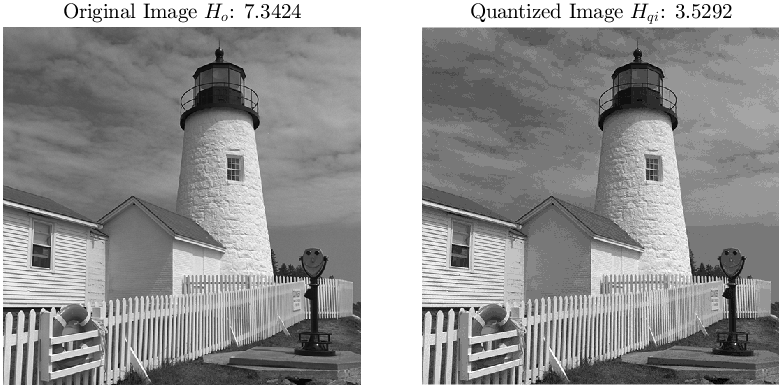
\includegraphics[width=1\textwidth]{QuantKodim.png}
    \centering
    \caption{Original and Quantized version of Kodim19}
    \label{fig:QuantKodim}
\end{figure}

\subsection{PSNR and Visual Quality}
The Peak Signal-to-Noise Ratio is a common metric used by many people to indicate the quality of a photo after some type of transformation. It works by comparing the transformed photo to a reference image, with low values indicating large differences from the reference and high values indicating that the two images are very similar. This can be calculated in MATLAB by calling the psnr function and passing the transformed image and the reference image as parameters. This yielded a result of 5.845 for the quantized image.

\noindent Visually the quantized image looks worse than the reference image. Due to the quantization, we lose the fine transitions between similar colors in the sky and on the walls. Instead, similar colors are replaced with one color, leading to the patches of homogeneous color we see in the image.

